	\documentclass[12pt]{article}
	\usepackage{hyperref}
	\usepackage{graphicx}
	\usepackage[T1]{fontenc}
	\usepackage[utf8]{inputenc}
	\usepackage{color}
	\usepackage[font=small,labelfont=bf]{caption}
	\usepackage[english]{babel}
	\usepackage{datetime}
	\usepackage{fancyhdr}
	\usepackage{lastpage}
	\usepackage{float}
	\pagestyle{fancy}
	\fancyhf{}
\addtolength{\oddsidemargin}{-3cm}
\addtolength{\evensidemargin}{-3cm}
\addtolength{\textwidth}{6cm}
\addtolength{\topmargin}{-3cm}
\addtolength{\textheight}{5cm}
	\usepackage{multicol}
	
	\newcommand\textline[4][t]{%
		\par\smallskip\noindent\parbox[#1]{.333\textwidth}{\raggedright\texttt{}#2}%
		\parbox[#1]{.333\textwidth}{\centering#3}%
		\parbox[#1]{.333\textwidth}{\raggedleft\texttt{#4}}\par\smallskip%
	}
	\rfoot{\textline[t]{}{Page \thepage \hspace{1pt} of \pageref{LastPage}}{}}
	\renewcommand{\today}{\thisdayofweekname\ \the\day\ \monthname\ \the\year}
	\title{Essay}
	\date{}
	\author{Trevisan Davide}
	\hypersetup{
		colorlinks=true,       % false: boxed links; true: colored links
		linkcolor=blue,          % color of internal links (change box color with linkbordercolor)
		citecolor=green,        % color of links to bibliography
		filecolor=blue,      % color of file links
		urlcolor=blue,
		filecolor=red,
		citecolor=blue,
	}
	\begin{document}
		\pagenumbering{arabic}
		
		
		
		\begin{titlepage}
			
			\newcommand{\HRule}{\rule{\linewidth}{0.5mm}} % Defines a new command for the horizontal lines, change thickness here
			
			\center % Center everything on the page
			
			%----------------------------------------------------------------------------------------
			%	HEADING SECTIONS
			%----------------------------------------------------------------------------------------
			
			\textsc{\LARGE University of Padova}\\[1.5cm] % Name of your university/college
			\textsc{\Large Computer and Network Security}\\[0.5cm] % Major heading such as course name
			
			%----------------------------------------------------------------------------------------
			%	TITLE SECTION
			%----------------------------------------------------------------------------------------
			
			\HRule \\[0.4cm]
			{ \huge insert-title-here}\\[0.3cm]
			 %TODO insert title 
			%Title of your document
			\HRule \\[1.5cm]
			
			%----------------------------------------------------------------------------------------
			%	AUTHOR SECTION
			%----------------------------------------------------------------------------------------
			
			\begin{minipage}{0.4\textwidth}
				\begin{flushleft} \large
					\emph{Students:}\\
					Davide Trevisan\\ % Your name
					Andrea Multineddu\\
				\end{flushleft}
			\end{minipage}
			~
			\begin{minipage}{0.4\textwidth}
				\begin{flushright}\large
					\emph{Registration number:} \\
					\textsc{1070686}\\ % matricola
					\textsc{matricola}\\
				\end{flushright}
			\end{minipage}\\[1cm]
			
			%----------------------------------------------------------------------------------------
			%	DATE SECTION
			%----------------------------------------------------------------------------------------
			
			{\large \today}\\[1cm] % Date, change the \today to a set date if you want to be precise
			
			%----------------------------------------------------------------------------------------
			%	LOGO SECTION
			%----------------------------------------------------------------------------------------
			
			
\includegraphics[scale=0.35]{Logo.png} % Include a department/university logo - this will require the graphicx package
			
			%----------------------------------------------------------------------------------------
			
			\vfill % Fill the rest of the page with whitespace
		\end{titlepage}
		
		\newpage

\begin{multicols}{2}
	\section*{Introduction}
	Nowadays the majority of browsers let users the possibility of customizing it in order to get a new feature o a new style of visualization to better match the taste of the single user.
	All of this is achievable through the existing extensions for modern browsers. But there is also the opposite situation in which a malicious user tries to get personal information using this extensions.
	
	\section*{Abstract}
	Google Chrome browser is known for it huge ammount of extensions that let users do almost everything they want, but there also malicious extensions that aim to steal personal information about the life, bank accounts and every other single piece of information of the users. In this paper we presents 3 extensions: ChromeLogger\cite{ChromeLogger}, Stealth Screenshot e Activity Logger;\\ \\
	ChromeLogger is a keylogger and form grabber for Google Chrome that runs as an extension.	
	ChromeLogger works by injecting javascript into all loaded web pages. The payload records keypresses using event listeners and saves them to Chrome's storage. Unlike other browser keyloggers, ChromeLogger runs natively in Chrome (on all OS's) without the need to install additional software.
	The form grabber works in a similar way. Javascript is injected and event listeners are added for all forms. When a form is submitted, its data is saved to ChromeLogger's storage. This allows form data transferred over SSL to be saved in plaintext.
	ChromeLogger's payload is written in pure JS and the log viewer is built using AngularJS.\\ \\
	Stealth Screenshot make screenshots of the active tab based on a timer and keep them until every opened tab is closed. Users can access with a combination of key to all screenshots taken during the session.\\ \\
	Activity Logger keep trace of all events related to extension and save them in Chrome storage. Users can check if there are installation, uninstallation, activation or deactivation of Chrome extension due to malicious code running in background.
\section*{How Chrome Extension works}
\subsection*{Background}
\subsubsection*{where to find an extension}
The Chrome Web Store is the official way for users
to find and install extensions, where the developers can publish it. They can also push out updates without any action
by the end-user.
In addition to the Chrome Web Store, extensions can
also be installed manually by a user or an external program.
Extension that are not downloaded through the official channel are flagged by Chrome when it starts	and the user is asked to disable them.
However, the user can whitelist the extension through the console.
\subsubsection*{Manually install an extension}
	Once you have all the source code of an extension in a folder, go to  \textsc{chrome://extensions} (or find it in the menu in more tools > extensions), then activate the developer mode on the top right of the page. To install the extension, you just have to indicate where is this folder on your computer clicking on load unpacked extention.
\subsection*{Permission}
Chrome requires extensions to list the
permissions needed to access the different parts of the
extension API. The complete list of the permissions and their interaction can be found on \href{https://developer.chrome.com/extensions/declare_permissions}{google developer page}.\\
Extensions must also specify a list of content scripts to indicate
JavaScript files that will run inside of the web page, because this is a powerful feature that allows an extension to be indistinguishable to the webpage behaviour. Besides the content scripts that
allow an extension to interact with a given page,
Chrome also allows extensions to run scripts in a
“background page” that often contain the
logic and state an extension needs for the entirety
of the browser session and do not have any visibility
to the user.\\
\section*{Activity Logger Extension}
\subsection*{Scope of the extension}
The extension aims to keep traces about the activities of other extensions and let the user know
about them through a dedicate page in which can check for every extension that are installed on the
Chrome browser. This logger keep traces of logs even if some extensions are unistalled. \\
The extension makes use of the following permission in the manifest file:
{\fontsize{10}{10}\selectfont
	\begin{itemize}
		\item  management
		\item  storage
		\item  unlimitedStorage
	\end{itemize}
}
\subsection*{How the extenssion work}
The extension at the browser start check the list of installed extension and updates the logs list with the one missing from it.
After this first check and update we create listener for the events related to extensions which are: 
{\fontsize{10}{10}\selectfont
	\begin{itemize}
		\item  chrome.management.onInstalled
		\item  chrome.management.onUninstalled
		\item  chrome.management.onEnabled
		\item  chrome.management.onDisabled
	\end{itemize}
}
Every time the user or some malicious code install, uninstall, enable or disable an extension a log of the triggered event is saved in the specific event log for the specific extension in the chrome storage.
The computation time is defined by the computation time of the Chrome search in his storage.
\subsection*{Limitations}
The main limitation to this extension can be reconducted to the limitation imposed by or absence of Chrome APIs.
At the moment we can just check the events described early in the paper, every other event defined in Chrome APIs and the presence or absence of listener for a specific event.
A better controll on browser activity could be achieved by adding APIs, for example that return the name of extension from which is running codes in response to a specific event.
\subsection*{Future work}
The final aims of this extension are to log every single activity of installed extensions and jasvacript scripts inside web pages in response to every event happening inside Chrome itself (like a modification inside the chrome storafe area) or the web pages visited by the user (the pression of a button) and let the user check these logs	in order to let users check some strange and unwanted activities caused by some malicious code. At this time, for what we have find out from our research on chrome API documentation we can just check if there is some code waiting a specific events that trigger it.
But this is also a double-edged weapon that can led to problems for privacy maintenance because let every user, capable of writing chrome extension the possibility to check every activity, but from the other hands let malicious users the possibility  on customizzable browsers to get knowledge about users routines, personal data and ad-hoc javascript code injection.
\section*{Stealth Screenshot Extension}
The source code of the extension we developed is downloadable \href{https://github.com/Trexy94/Stealth-screenshot}{here}
\subsection*{Scope of the extension}
the scope of the stealth screenshot extension is to create a small prototype of an extension that catch screenshot in a regular interval with the minimum possible user interaction and obviously giving it back.
\subsubsection*{Activation and screenshot collection}
The extension uses the relatively new tab APIs given by chrome too take screenshot.
The extension makes use of the "storage", "tabs", "all\_urls;", "unlimitedStorage", "activeTab" permissions in his manifest file. The extension works in a simple way: it triggers on a browser event, in this case the click on the icon of the extension, but there are other possibilities: we tested that there are no simple ways to take screenshot without no interaction, because the security policy of the API doesn't allow to take a scrrenshot without some kind of events, presuming that the user should be aware of what is happening; not triggering any event returns only null.
Once triggered, the extension schedule all the future screenshot through the Javascript setTimeout method: this allows to take screenshot for hours, with only the need for a click to start.
The screenshot are stored in an array visible to all the extention methods.
\subsubsection*{Screenshot retrival}
The screenshot can be collected in two ways in the wxtension we developed:
through a combination of key for retriving all screenshots (we programmed it on Ctrl+Shift+Y) or writing "show" in the omnibox, pressing "tab" and writing in the omnibox the number of screenshot to show (starting from the last one).
\subsubsection*{Performance}
We tested that the extension is able to take screenshot with a interval of 1 minute for more than 2 hours without losing any screenshot.
The application occupy less of 50MB of RAM for an hour of screenshots taken every minute. The impact on the CPU is negligible.
Screenshot retrival through the kay combo however can  crash chrome, although it never happened in our PC because of the great performance (we had an Intel i5 6400, with 8GB of DDR4 memory and SSD), but it got freezed for some seconds.
\subsection*{Limitations}
The major limitation of this extension is that the screenshot only lives until the extension is active: this implies that closing all the windows of chrome completely deletes the screenshot taken.
This is a consequence of how the API and the chrome sandbox works. We at the moment found no way to get around it, but we are pretty confident that is possible to save those screenshots, but for our lack of knowledge we are not able at the moment to demonstrate it.
\subsection*{Future work}
Possible future works will focus on find a way to save those screenshot.
The application should also be rewritten without the tab API, to avoid of the limitation of it.
Javascript inject the code for the screenshot or use it for simulate the right events should do the work, but the time and the train needed to do it made impossible for us to test it for this paper.
\section*{conclusions}
All the solution we have presented in thispaper makes use of the most used chrome permission, as already stated in the HULK paper\cite{HULK}
\begin{figure}[H]
	\begin{center}
		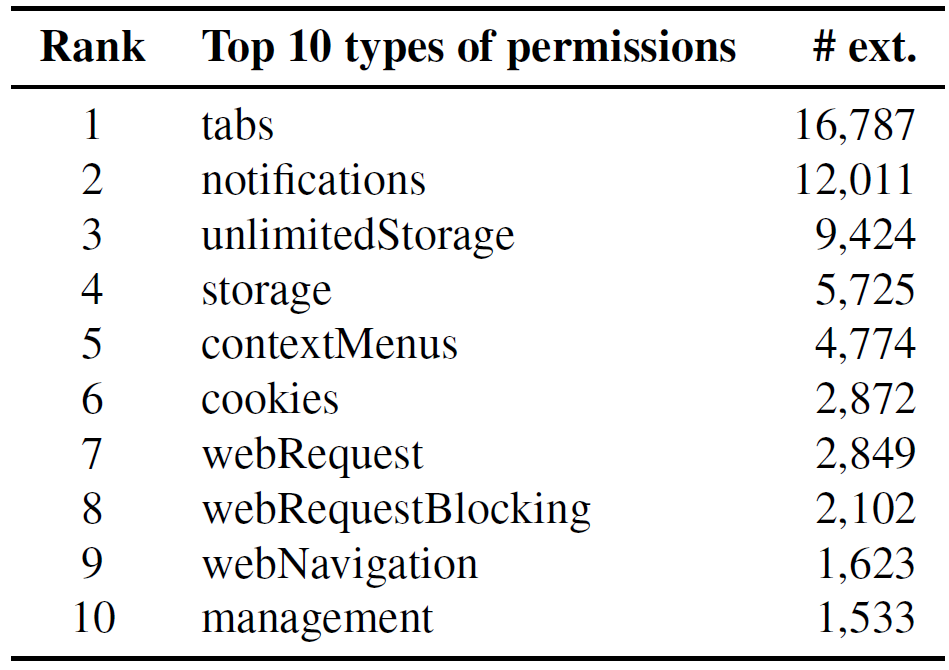
\includegraphics[width=6cm]{permission.png}
		\caption{The top 10 permissions found in the manifest
			files for all extensions we ran. Extensions can include			
			more than one permission.}
	\end{center}
\end{figure}
As shown in the screenshot extension, taking screenshot without user consensus should not be allowed to the API (just a popup should be enough)
\begin{thebibliography}{2}
	\bibitem{ChromeLogger}
	Eric Zhang,\\
	\emph{ChromeLogger},\\
A keylogger and form grabber for Google Chrome that runs as an extension.\\
\href{https://github.com/Xeroday/ChromeLogger}{ChromeLogger}\\
\href{https://www.ericzhang.me/projects/chromelogger/}{referring site}

\bibitem{HULK}
\emph{Hulk: Eliciting Malicious Behavior in Browser Extensions}\\
Alexandros Kapravelos, Chris Grier, Neha Chachra, Christopher Kruegel
Giovanni Vigna, Vern Paxson,
UC Santa Barbara,
UC Berkeley, 
UC San Diego and 
International Computer Science Institute\\
\emph{23rd USENIX Security Symposium.}\\
\href{https://www.usenix.org/system/files/conference/usenixsecurity14/sec14-paper-kapravelos.pdf}{Paper}\\	
\end{thebibliography}
\end{multicols}
 
\end{document}